% Flowchart
% Author: Stefan Kottwitz
% https://www.packtpub.com/hardware-and-creative/latex-cookbook
\documentclass[border=20pt]{article}
\date{}
\usepackage{color}
% \usepackage[vmargin=3cm,width=15cm]{geometry}
\usepackage{tikz}
\usetikzlibrary{matrix,calc,shapes}
\tikzset{
  treenode/.style = {shape=rectangle, 
                     draw, anchor=center,
                     text width=5em, align=center,
                     top color=white, bottom color=blue!20,
                     inner sep=1ex},
  decision/.style = {treenode, diamond, inner sep=0pt},
  root/.style     = {treenode, font=\Large, bottom color=red!30},
  env/.style      = {treenode, font=\ttfamily\normalsize},
  finish/.style   = {draw,top color=white, bottom color=green!20, font=\sffamily\large},
  dummy/.style    = {draw,top color=white, rounded corners, bottom color=orange!20, font=\sffamily\large}
}
\newcommand{\yes}{edge node [above] {yes}}
\newcommand{\no}{edge  node [left]  {no}}
\newcommand{\links}[1]{edge  node [left]  {#1}}
\newcommand{\rechts}[1]{edge  node [right]  {#1}}
\newcommand{\oben}[1]{edge  node [above]  {#1}}
\newcommand{\unten}[1]{edge  node [below]  {#1}}

\title{Reviewing of edited volumes}
\begin{document}  
\pagestyle{empty} 
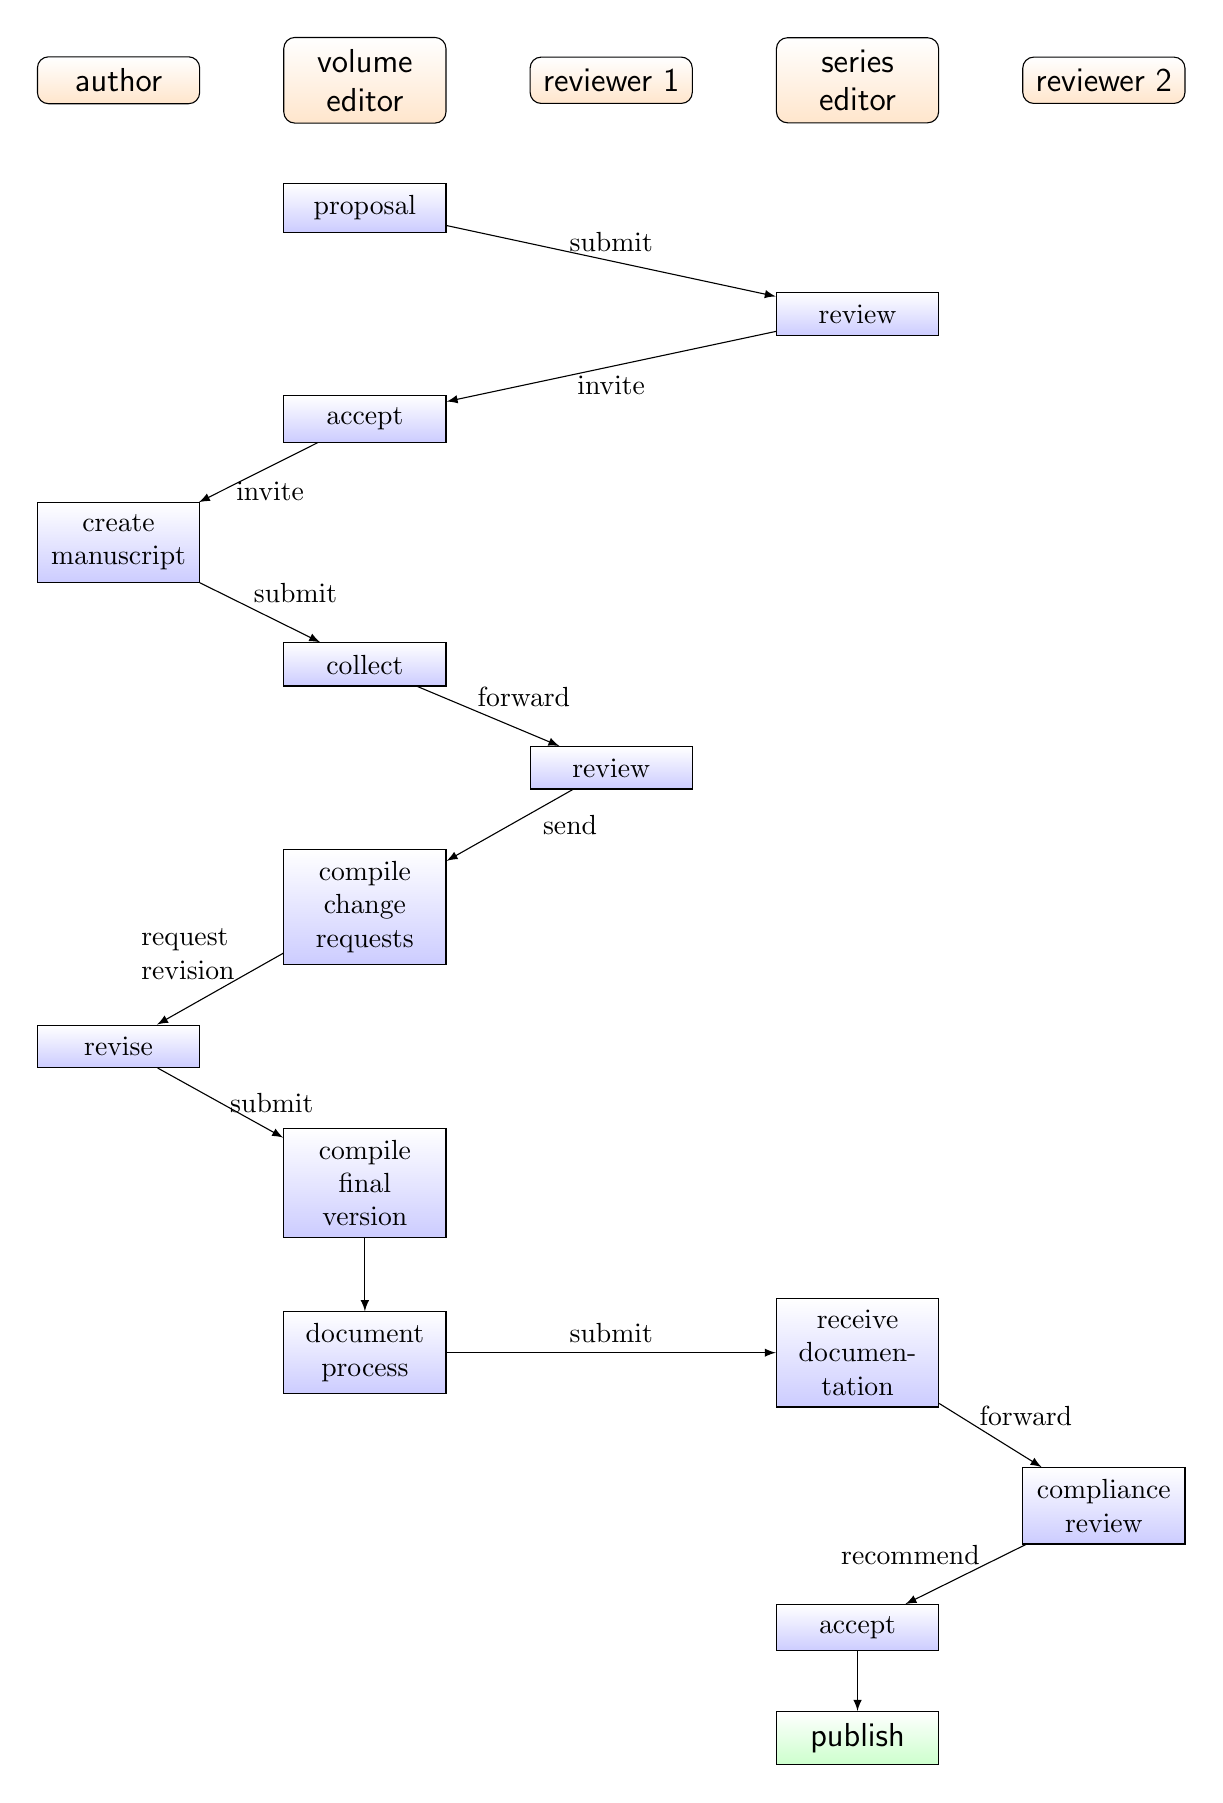
\begin{tikzpicture}[-latex]
  \matrix (chart)
    [
      matrix of nodes,
      column sep      = 3em,
      row sep         = 5ex,
      column 1/.style = {nodes={treenode}},
      column 2/.style = {nodes={treenode}},
      column 3/.style = {nodes={treenode}},
      column 4/.style = {nodes={treenode}},
      column 5/.style = {nodes={treenode}},
      row 1/.style = {nodes={dummy}}
%       column 2/.style = {nodes={env}}
    ]
    {
      author  & volume editor & reviewer~1 & series editor & reviewer~2\\
			& proposal      &           &               &           \\
			& 		 &           &     review        &           \\
			& accept            &           &               &           \\
	create manuscript 	&               &           &               &           \\
			& collect       &           &               &           \\
			&               &  review       &               &           \\
			& compile change requests & &               &           \\
	revise		&               &           &               &           \\
			&    compile final version    &           &        &           \\
			&    document process		    &           &    receive documentation    &           \\
			&               &           &     	     &  compliance review        \\
			&               &           &    accept    &           \\
			&               &            & |[finish]| publish \\
    };
  \draw
    (chart-2-2) \oben{submit\hspace{9mm}} (chart-3-4)
    (chart-3-4) \unten{invite} (chart-4-2)
    (chart-4-2) \unten{\hspace{3mm}invite} (chart-5-1)
    (chart-5-1) \oben{\hspace{9mm}submit} (chart-6-2)
    (chart-6-2) \oben{\hspace{9mm}forward} (chart-7-3)
    (chart-7-3) \rechts{\hspace{3mm}send} (chart-8-2)
    (chart-8-2) \oben{\parbox{2cm}{request\\ revision}\hspace{13mm}} (chart-9-1)
    (chart-9-1) \rechts{submit~~~~} (chart-10-2)
    (chart-10-2) edge (chart-11-2)
    (chart-11-2) \oben{submit} (chart-11-4)
    (chart-11-4) \oben{\hspace{9mm}forward} (chart-12-5)
    (chart-12-5) \oben{recommend\hspace*{14mm}} (chart-13-4)
    (chart-13-4) edge (chart-14-4); 
\end{tikzpicture}   
\end{document}
\section*{Two reviews-systems}
The two review system comes in two kinds. The first kind is the "Early Two Reviews System", the second kind is the "Late Two Reviews System".

\subsection*{Early Two Reviews System}
 In the Early Two Reviews System, the VE submits all initial submissions they wish to include together with the reviews to the SE. The SE then gets reviews for that material and decides whether to accept the submission. The early two review system is similar to the Compliance System in that the reviewer gets to see the first round reviews. If this second-level reviewer recommends acceptance, the SE informs the VE that the first-level reviews can be sent to the authors. The book counts as accepted. The incorporation of the changes by the authors is subsequent to this. The final version of the edited volume is sent to the Series editor and counts as accepted. In that sense, the Early Two Review System is similar to the Delegated System because a rejection is no longer possible at that point in time. 


\subsection*{Late Two Reviews System}
The late two reviews system differs from the Early Two Reviews System in that the version sent to the second tier reviewers is not the initial one, but the one which already incorporates the first-tier reviewers' comments. This will make it easier for the second-level reviewer to judge the papers, but it can also lead to frustration if the book ends up being turned down and the authors' work on revising the papers based on the first-tier comments was for nothing. Second level reviewers in the Late Two Reviews System only judge the global scientific merit of the final volume. A judgment of the procedure is then not necessary.


% \begin{figure}
% \begin{tikzpicture}[-latex]
%   \matrix (chart)
%     [
%       matrix of nodes,
%       column sep      = 3em,
%       row sep         = 5ex,
%       column 1/.style = {nodes={treenode}},
%       column 2/.style = {nodes={treenode}},
%       column 3/.style = {nodes={treenode}},
%       column 4/.style = {nodes={treenode}},
%       column 5/.style = {nodes={treenode}},
%       row 1/.style = {nodes={dummy}}
% %       column 2/.style = {nodes={env}}
%     ]
%     {
%       author  & volume editor & reviewer~1 & series editor & reviewer~2\\ 
% 	create manuscript 	&               &           &               &           \\
% 			& collect       &           &               &           \\
% 			&               &  review       &               &           \\
% 			& select papers & &               &           \\
% 			& compile documentation & &    receive           &           \\ 
% 			&               &           &     	     &  evaluate content        \\
% 			&               &           &     	     &  evaluate procedure        \\
% 			&  compile change requests             &           &    decide    &           \\ 
% 	revise		&               &           &               &           \\
% 			&    compile final version    &           &     accept   &           \\ 
% 			&               &            & |[finish]| publish \\
%     };
%   \draw 
%     (chart-2-1) \oben{\hspace{9mm}submit} (chart-3-2)
%     (chart-3-2) \oben{\hspace{9mm}forward} (chart-4-3)
%     (chart-4-3) \rechts{\hspace{3mm}send} (chart-5-2) 
%     (chart-5-2) edge (chart-6-2) 
%     (chart-6-2) \oben{\hspace{3mm}submit} (chart-6-4) 
%     (chart-6-4) \rechts{\hspace{3mm}forward} (chart-7-5) 
%     (chart-7-5)  edge (chart-8-5) 
%     (chart-8-5) \rechts{\hspace{3mm}send} (chart-9-4) 
%     (chart-9-4) \oben{\hspace{3mm}forward} (chart-9-2)
%     (chart-9-2) \rechts{\hspace{3mm}request revisions} (chart-10-1)
%     (chart-10-1) \links{\hspace{3mm}submit} (chart-11-2)
%     (chart-11-2) \oben{\hspace{3mm}submit} (chart-11-4) 
%     (chart-11-4) edge (chart-12-4) 
% ;
% \end{tikzpicture} 
% \caption{Early two review system}
% \end{figure}
 
% 
% \begin{figure}
% \begin{tikzpicture}[-latex]
%   \matrix (chart)
%     [
%       matrix of nodes,
%       column sep      = 3em,
%       row sep         = 5ex,
%       column 1/.style = {nodes={treenode}},
%       column 2/.style = {nodes={treenode}},
%       column 3/.style = {nodes={treenode}},
%       column 4/.style = {nodes={treenode}},
%       column 5/.style = {nodes={treenode}},
%       row 1/.style = {nodes={dummy}}
% %       column 2/.style = {nodes={env}}
%     ]
%     {
%       author  & volume editor & reviewer~1 & series editor & reviewer~2\\ 
% 	create manuscript 	&               &           &               &           \\
% 			& collect       &           &               &           \\
% 			&               &  review       &               &           \\
% 			& compile change requests & &               &           \\
% 	revise		&               &           &               &           \\
% 			&    compile final version    &           &        &           \\
% 			&    document process		    &           &    receive documentation    &           \\
% 			&               &           &     	     &  evaluate content        \\ 
% 			&               &           &    accept    &           \\
% 			&               &            & |[finish]| publish \\
%     };
%   \draw 
%     (chart-2-1) \oben{\hspace{9mm}submit} (chart-3-2)
%     (chart-3-2) \oben{\hspace{9mm}forward} (chart-4-3)
%     (chart-4-3) \rechts{\hspace{3mm}send} (chart-5-2)
%     (chart-5-2) \oben{\parbox{2cm}{request\\ revision}\hspace{13mm}} (chart-6-1)
%     (chart-6-1) \rechts{submit~~~~} (chart-7-2)
%     (chart-7-2) edge (chart-8-2)
%     (chart-8-2) \oben{submit} (chart-8-4) 
%     (chart-8-4) \rechts{forward} (chart-9-5) 
%     (chart-9-5) \oben{recommend\hspace*{14mm}} (chart-10-4)
%     (chart-10-4) edge (chart-11-4); 
% \end{tikzpicture}  
% \caption{Late two review system}
% \end{figure}

\end{document}